\documentclass[a4paper]{article}

\usepackage[utf8x]{inputenc}
\usepackage[russian, english]{babel}
\usepackage{cmap}
\usepackage{dsfont}
\usepackage{amsmath}
\usepackage{amssymb}
\usepackage{comment}
\usepackage{graphicx}
\usepackage{caption}
\usepackage{geometry}
\usepackage{easyeqn}
\usepackage{bbm}

\pagestyle{plain}

\title{Gaussian Process in Active Learning for Classification}
\author{Daria Kotova, Maxim Panov}

\begin{document}

\maketitle

\setlength{\marginparwidth}{2cm}
\selectlanguage{english}

\begin{abstract}

There is a working file with description of what we are doing.

\end{abstract}

\section{Gaussian Process}

In this section we briefly review the definition of gaussian process and some important equations connected with it. A comprehensive overview of gaussian processes is presented in \cite{gp}. \\
{\em  Gaussian process} $f\left(x\right)$ -- stochastic process (a collection of random variables indexed by time or space), such that every finite collection of those random variables has a multivariate normal distribution. Here $x \in \mathbb{R}^D$, where $D$ - arbitrary natural number. \\
Gaussian process is defined by mean and covariance functions. Often mean function is chosen as constant 0. We introduce the notation:
\begin{align*}
m\left(x\right) & = \mathds{E}\left[ f\left(x\right) \right] = 0, \\
K\left(x, x'\right) & = \mathds{E} \left[ \left(f\left(x\right) - m\left(x\right)\right) \left(f\left(x'\right) - m\left(x'\right)\right)\right].
\end{align*}
\paragraph{Regression.} We want to get posterior on process $f\left(x\right)$, having observed points $X$. Prior is defined by:
\begin{EQA}[c]
\begin{pmatrix}
f \\
f_{*}
\end{pmatrix} \sim \mathcal{N}
\left(
0, 
\begin{pmatrix}
K(X, X) & K(X, X_{*}) \\
K(X_{*}, X) & K(X_{*}, X_{*})
\end{pmatrix}\right),
\end{EQA}
where $*$ corresponds to the test set. With Bayes formula and some calculations we show that posterior will look like:
\begin{EQA}[c]\label{aposterior}
\left( f_{*} | X, X_{*}, f \right) \sim \mathcal{N} (\hat{f}, \hat{\sigma}^2),
\end{EQA}
\begin{align*}
\text{where } \hat{f} & = K(X_{*}, X)K(X, X)^{-1}f \text{ -- mean function,} \\
\hat{\sigma}^2 & = K(X_{*}, X_{*}) - K(X_{*},X)K(X, X)^{-1}K(X,X_{*})) \text{ -- covariance function.}
\end{align*} \\
The reader can notice that interpretation of this result for covariance function is quite intuitive: $K(X_{*}, X_{*})$ is prior covariance and positive term, corresponding to new information, is substracted from prior knowledge.\\
To sum up, in regression case gaussian process give us not only mean, but also variance -- the measure of uncertainty in a giving point. This property is advantage of gaussian proccess. However, we should point out that matrix inversion in \eqref{aposterior} is extremely time consuming.

\section{Active Learning}

Now let's move on to basics of active learning approach. It is based on an assumption that model will give better results having less training points, if we allow it to choose points to train on by itself. \\
The algorithm is quite simple: the model chooses the next point which label it wants to get. Then ask an "oracle" for the label and somehow incorporates new knowledge. Then it repeats all the steps till some condition for stopping. Review of active learning can be found in \cite{generalav}. \\ 
We will consider pool-based sampling, which assumes that there is a small set of labeled data $\mathcal{L} = (x_1, ..., x_n)$ and a large pool of unlabeled data $\mathcal{U}$ available. New points are selectively drawn from the pool taking into account some acquisition function $g(u)$. Often new point $u^*$ delivers maximum of $g(u)$. This approach is also illustrated in Fig.\ref{activelearning}.\\
\begin{figure}[h]
\vspace{0 cm}
\center{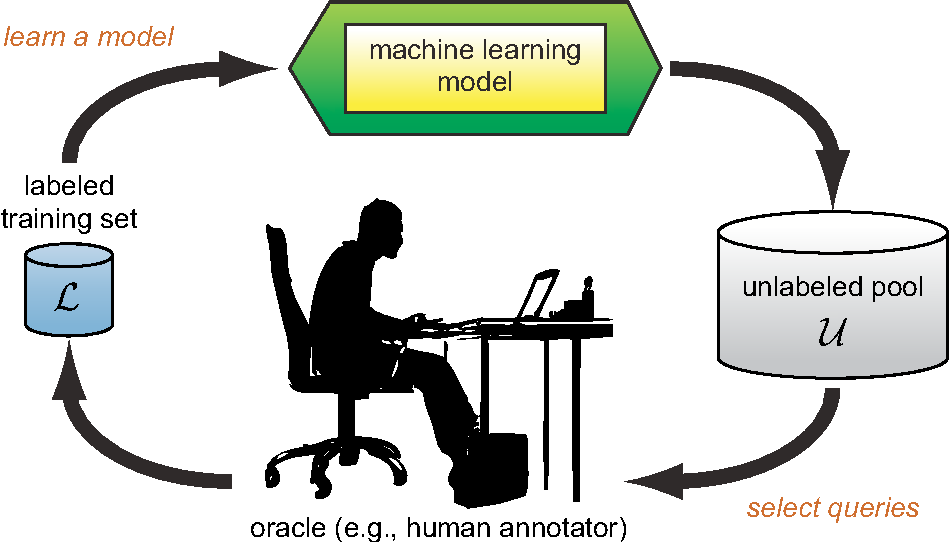
\includegraphics[scale = 0.25]{definition1.png}}
\caption{Illustration of active learning algorithm using pool-based method.}
\label{activelearning}
\end{figure}
In this work we tried different $g(u)$. As a reference we used the work \cite{av} where general criterion and some specific variants were introduced. Now we will consider results of this work.\\
Let $f$ be the minimum norm function that interpolates labeles examples. Define $f_t^u(x)$ is the minimum norm interpolating function based on $\mathcal{L}$ and the point $u \in \mathcal{U}$. To get $f_t^u(x)$ we suppose that $u$ has label $t$ (since in supervised learning we have to have labeles for put points). Then our $g(u)$ can be presented as (both variants are possible):
\begin{EQA}[c]\label{score}
g(u) = \|f^u_t(v)\|, \ g(u) = \|f^u_t(v)-f(v)\|.
\end{EQA}
%Пусть $f$ -- функция, интерполирующая примеры из тренировочного множества, с минимальной нормой (это условие получено из опытов \cite{minnorm} -- такие модели, как правило, имеют хорошие обощающие свойства). Определим $f_t^u(x)$ - как функцию, интерполирующую примеры из тренировочного множества, объединенного с точкой $u \in \mathcal{U}$ с меткой $t$, с минимальной нормой. Метку $t(u)$ будем выбирать одним из следующих способов:
\begin{comment}
\begin{equation}\label{t}
t^{(1)}(u) = argmin_{t\in\{-1,1\}}\|f_t^u(x)\|, \ t^{(2)}(u) = 
 \begin{cases}
   +1 \ \text{if} \ f(u) \geq 0, 
   \\
   -1  \ \text{if} \ f(u) < 0
 \end{cases}
\end{equation}
%Определив $t(u)$, положим $f^u(x) = f^u_{t(u)}(x)$. Введем так же $score$-функции:
\begin{equation}\label{score}
score^{(1)}(u) = \|f^u(x)\|, \ score^{(2)}(u) = \|f^u(x)-f(x)\|,
\end{equation}
%В первом случае больший $score$ получит менее гладкая функция, во втором -- та функция, которая наиболее сильно отличается от предыдущей интерполяции. Ожидается, что точка с большим $score$-ом наиболее информативная.\\
%Тогда следующая точка для получения метки есть $$u^* = argmax_{u \in \mathcal{U}} score(u).$$
%В выражениях \eqref{t} и \eqref{score} намеренно не определена конкретная норма для свободы в выборе различных вариаций $score$-функций. Если эти нормы выбраны одинаковы и выбрана первая $score$-функция, то новая точка $u^*$ выбирается такой, что
\begin{equation}
\|f^{u^*}(x)\| = max_{u \in \mathcal{U}}min_{t\in\{-1,1\}} \|f_t^u(x) \|.
\end{equation}
\end{comment}

\section{Criteria}
Here we compare 6 different ways to choose new point $u^*$ from unlabeled data $\mathcal{U}$. Having assumed that $u^* = \underset{u \in \mathcal{U}}{argmax} ( g(u))$, we change $g(u)$ and compare results.
\begin{enumerate}
\item {\em Random   } -- just to check if results are adequate (rand).

\item {\em Variance } -- new point corresponds to the maximum of variance:
\begin{EQA}[c] 
g(u) = \hat{\sigma}^2(u) \text{\ (mvar).}
\end{EQA}

\item {\em 2-norm   } -- the criterion was introduced in \cite{av}. A new point is the argmax of: 
\begin{EQA}[c] 
g(u) = \|f^u_t(v)-f(v)\|_{\mathcal{U}} = \sqrt{\sum\limits_{v \in \mathcal{U}}(f^u_t(v)-f(v))^2} \text{\ (sqsm).}
\end{EQA}

\item {\em RKHS-norm} -- this criterion was also introduced in \cite{av}. However, we want to provide more comprehensive inference here: 
\begin{EQA}[c] 
g(u) = \|f^u_t(v)\|_{\mathcal{H}} = \vec{\widetilde{y}^T_t} \widetilde{K} \vec{\widetilde{y}_t} \text{\ computed with RKHS-norm (RKHS).}
\end{EQA}
Let's infer the $\|f^u_t(v)\|_{\mathcal{H}}$. \ Let $\widetilde{K} = 
\begin{pmatrix}
K			& \vec{a} \\
\vec{a}^T	& b
\end{pmatrix}
$, where $b = K(u, u), \vec{a} = [K(x_1, u), ... , K(x_n, u)]^T$.
Using Schur complement formula we have $\widetilde{K}^{-1}$ as:
\begin{EQA}
\widetilde{K}^{-1} & = &
\begin{pmatrix}
 K^{-1} + K^{-1}\vec{a}(b-\vec{a}^TK^{-1}\vec{a})^{-1}\vec{a}^TK^{-1} & 
-K^{-1}\vec{a}(b-\vec{a}^TK^{-1}\vec{a})^{-1} \\
-(b-\vec{a}^TK^{-1}\vec{a})^{-1}\vec{a}^TK^{-1} & (b-\vec{a}^TK^{-1}\vec{a})^{-1} \\
\end{pmatrix} 
\\ 
& = &\begin{pmatrix}
K^{-1} + \frac{K^{-1}\vec{a}\vec{a}^TK^{-1}}{b-\vec{a}^TK^{-1}\vec{a}} & 
\frac{-K^{-1}\vec{a}}{b-\vec{a}^TK^{-1}\vec{a}} \\
\frac{-\vec{a}^TK^{-1}}{b-\vec{a}^TK^{-1}\vec{a}} & \frac{1}{b-\vec{a}^TK^{-1}\vec{a}} \\
\end{pmatrix} .
\end{EQA}

Then $\|f^u_t(v)\|$ turns into:
\begin{EQA}
	\|f^u_t(v)\| & = & \vec{y}^TK^{-1}\vec{y} + \vec{y}^T \frac{K^{-1}\vec{aa}^TK^{-1}}{b - \vec{a}^TK^{-1}\vec{a}}\vec{y} - 2t\vec{y}^TK^{-1}\frac{\vec{a}}{b} -  2t\vec{y}^T \frac{K^{-1}\vec{aa}^TK^{-1}}{b - \vec{a}^TK^{-1}\vec{a}}\frac{\vec{a}}{b} + \frac{1}{b - \vec{a}^TK^{-1}\vec{a}} 
    \\
    & = & \vec{y}^TK^{-1}\vec{y} + \frac{\left(\vec{y}^TK^{-1}\vec{a}\right)^2}{b - \vec{a}^TK^{-1}\vec{a}} - 2t\frac{\vec{y}^TK^{-1}\vec{a}}{b}\left(1 + \frac{\vec{a}^TK^{-1}\vec{a}}{b - \vec{a}^TK^{-1}\vec{a}}\right) + \frac{t^2}{b - \vec{a}^TK^{-1}\vec{a}} 
    \\
    & = & \vec{y}^TK^{-1}\vec{y} + \frac{\left(\vec{y}^TK^{-1}\vec{a}\right)^2}{b - \vec{a}^TK^{-1}\vec{a}} - \frac{2t\left(\vec{y}K^{-1}\vec{a}\right)}{b - \vec{a}^TK^{-1}\vec{a}} + \frac{t^2}{b - \vec{a}^TK^{-1}\vec{a}} 
    \\
    & = & \vec{y}^TK^{-1}\vec{y}  + \frac{\left(\vec{y}^TK^{-1}\vec{a} - t\right)^2}{b - \vec{a}^TK^{-1}\vec{a}} = \vec{y}^TK^{-1}\vec{y}  + \frac{\left(f(u) - y(u)\right)^2}{b - \vec{a}^TK^{-1}\vec{a}}.
\end{EQA}
That means 
\begin{EQA}[c]
g(u) = \|f^u_t(v)\|_{\mathcal{H}} = \vec{\widetilde{y}^T_t} \widetilde{K} \vec{\widetilde{y}_t} = \|f(v)\|_{\mathcal{H}} + \frac{(1 - t \cdot f(u))^2}{b - \vec{a}^T K^{-1} \vec{a}},
\end{EQA}
It is important to emphasize that denominator here is the posterior variance of the model at the point $u$ (see \eqref{aposterior}).

\item {\em RKHS-norm $\cdot$ variance} -- RKHS-norm turns out to have too huge values. Multiplying by variance allows solve the problem and also make quality of the criterion better. This idea was introduced in \cite{Hvar} (Hvar). 
\begin{EQA}[c]
g(u) = (\|f^u_t(v)\| - \|f(v)\|_{\mathcal{H}}) \cdot \hat{\sigma}^2(u) = (1 - t \cdot f(u))^2.
\end{EQA}
\item {\em 2-norm in formula} -- in sqsm we directly learned new model for each $u$. However, it can be simplified using previous knowledge (l2fm): \\
Let $\widetilde{a} = \begin{pmatrix}
\vec{a} \\
K(u,v)
\end{pmatrix} $ . Where $u$ is the new point and $v \in \mathcal{U}$ is the point we calculate $f(v)$ for. \\
Let's compute difference $f^u_t(v) - f(v)$:\\
\begin{EQA}
	f^u_t(v) - f(v) & = & 	\vec{\widetilde{a}}^T\widetilde{K}^{-1}\vec{\widetilde{y}} - \vec{a}^TK^{-1}\vec{y} 
	\\ 
	& = & \begin{pmatrix}
\vec{a}^T & K(u,v)
\end{pmatrix}
\begin{pmatrix}
K^{-1} + \frac{K^{-1}\vec{a}\vec{a}^TK^{-1}}{b-\vec{a}^TK^{-1}\vec{a}} & 
\frac{-K^{-1}\vec{a}}{b-\vec{a}^TK^{-1}\vec{a}} \\
\frac{-\vec{a}^TK^{-1}}{b-\vec{a}^TK^{-1}\vec{a}} & \frac{1}{b-\vec{a}^TK^{-1}\vec{a}} \\
\end{pmatrix}
\begin{pmatrix}
\vec{y} \\
t
\end{pmatrix} - \vec{a}^TK^{-1}\vec{y} 
	\\ 
	& = & \frac{(\vec{a}^TK^{-1}\vec{a} - K(u,v))(\vec{a}^TK^{-1}\vec{y} - t)}{b - \vec{a}^TK^{-1}\vec{a}}.\\	
g(u) & = & \|f^u_t(v)-f(v)\|_{\mathcal{U}} = \sqrt{\sum\limits_{v \in \mathcal{U}}(f^u_t(v)-f(v))^2} \\
	& = & \sqrt{\sum\limits_{v \in \mathcal{U}}\left( 
	\frac{(\vec{a}^TK^{-1}\vec{a} - K(u,v))(\vec{a}^TK^{-1}\vec{y} - t)}{b - \vec{a}^TK^{-1}\vec{a}}
	\right)^2}
\end{EQA}
\end{enumerate}

\begin{thebibliography}{}

\bibitem[1]{Hvar}
Burnaev E., Panov M. (2015) 
Adaptive Design of Experiments Based on Gaussian Processes. In: Gammerman A., Vovk V., Papadopoulos H. (eds) Statistical Learning and Data Sciences. SLDS 2015. 
Lecture Notes in Computer Science, vol 9047. Springer, Cham

\bibitem[2]{gp}
C. E. Rasmussen, C. K. I. Williams, 
Gaussian Processes for Machine Learning, 
the MIT Press, 2006, ISBN 026218253X

\bibitem[3]{av}
Mina Karzand, Robert D. Nowak:
Active Learning in the Overparameterized
and Interpolating Regime
arXiv preprint arXiv:1905.12782,2019

\bibitem[4]{generalav}
Burr Settles. 
Active Learning Literature Survey.  
2010.

\end{thebibliography}

\end{document}
